% Copyright 2004 by Till Tantau <tantau@users.sourceforge.net>.
%
% In principle, this file can be redistributed and/or modified under
% the terms of the GNU Public License, version 2.
%
% However, this file is supposed to be a template to be modified
% for your own needs. For this reason, if you use this file as a
% template and not specifically distribute it as part of a another
% package/program, I grant the extra permission to freely copy and
% modify this file as you see fit and even to delete this copyright
% notice. 

\documentclass{beamer}

% There are many different themes available for Beamer. A comprehensive
% list with examples is given here:
% http://deic.uab.es/~iblanes/beamer_gallery/index_by_theme.html
% You can uncomment the themes below if you would like to use a different
% one:
%\usetheme{AnnArbor}
%\usetheme{Antibes}
%\usetheme{Bergen}
%\usetheme{Berkeley}
%\usetheme{Berlin}
%\usetheme{Boadilla}
%\usetheme{boxes}
%\usetheme{CambridgeUS}
%\usetheme{Copenhagen}
%\usetheme{Darmstadt}
%\usetheme{default}
%\usetheme{Frankfurt}
%\usetheme{Goettingen}
%\usetheme{Hannover}
%\usetheme{Ilmenau}
%\usetheme{JuanLesPins}
%\usetheme{Luebeck}
\usetheme{Madrid}
%\usetheme{Malmoe}
%\usetheme{Marburg}
%\usetheme{Montpellier}
%\usetheme{PaloAlto}
%\usetheme{Pittsburgh}
%\usetheme{Rochester}
%\usetheme{Singapore}
%\usetheme{Szeged}
%\usetheme{Warsaw}

\title{Body measurements using Computer Vision}

% A subtitle is optional and this may be deleted
%\subtitle{Optional Subtitle}

\author{Ankesh Gupta \and Krunal Shah \and Saket Dingliwal}
% - Give the names in the same order as the appear in the paper.
% - Use the \inst{?} command only if the authors have different
%   affiliation.

%\institute[Universities of Somewhere and Elsewhere] % (optional, but mostly needed)
% {
%   \inst{1}%
%   Department of Computer Science\\
%   University of Somewhere
%   \and
%   \inst{2}%
%   Department of Theoretical Philosophy\\
%   University of Elsewhere}
% - Use the \inst command only if there are several affiliations.
% - Keep it simple, no one is interested in your street address.

%\date{Conference Name, 2013}
% - Either use conference name or its abbreviation.
% - Not really informative to the audience, more for people (including
%   yourself) who are reading the slides online

%\subject{Theoretical Computer Science}
% This is only inserted into the PDF information catalog. Can be left
% out. 

% If you have a file called "university-logo-filename.xxx", where xxx
% is a graphic format that can be processed by latex or pdflatex,
% resp., then you can add a logo as follows:

% \pgfdeclareimage[height=0.5cm]{university-logo}{university-logo-filename}
% \logo{\pgfuseimage{university-logo}}

% Delete this, if you do not want the table of contents to pop up at
% the beginning of each subsection:

% Let's get started
\begin{document}

\begin{frame}
  \titlepage
\end{frame}

\begin{frame}{Outline}
  \tableofcontents
  % You might wish to add the option [pausesections]
\end{frame}

% Section and subsections will appear in the presentation overview
% and table of contents.
\section{Problem Statement}
\section{Pipeline}

\section{Algorithm- Techniques/Methods used}
\subsection{Corrections - Affine and Metric}
\subsection{Segmentation - Green Screen Segmentation}
\subsection{Self designed heuristics for automatic detection of body parts}

\section{Resuts}
\subsection{Comparison with 3D skeleton method using Kinect}

\section{Future Scope}

\begin{frame}{Problem Statement}
  \begin{itemize}
  \item Determine the body measurements of a person as accurately as possible from a set of images
  \end{itemize}
  \bigskip
  \begin{itemize}
  \item To do so we need atleast one length in the image with known metric 
  \end{itemize}
\end{frame}

\begin{frame}{Uses}
  \begin{itemize}
  \item Boost customized online-cloth trade and commerce.
  \bigskip
  \item Help build virtual-trial rooms, because it solves the easier problem of cloth fitting on person.
  \bigskip
  \item Serve as a virtual tailor.
  \end{itemize}
\end{frame}


\begin{frame}{Pipeline}
\begin{figure}[h]
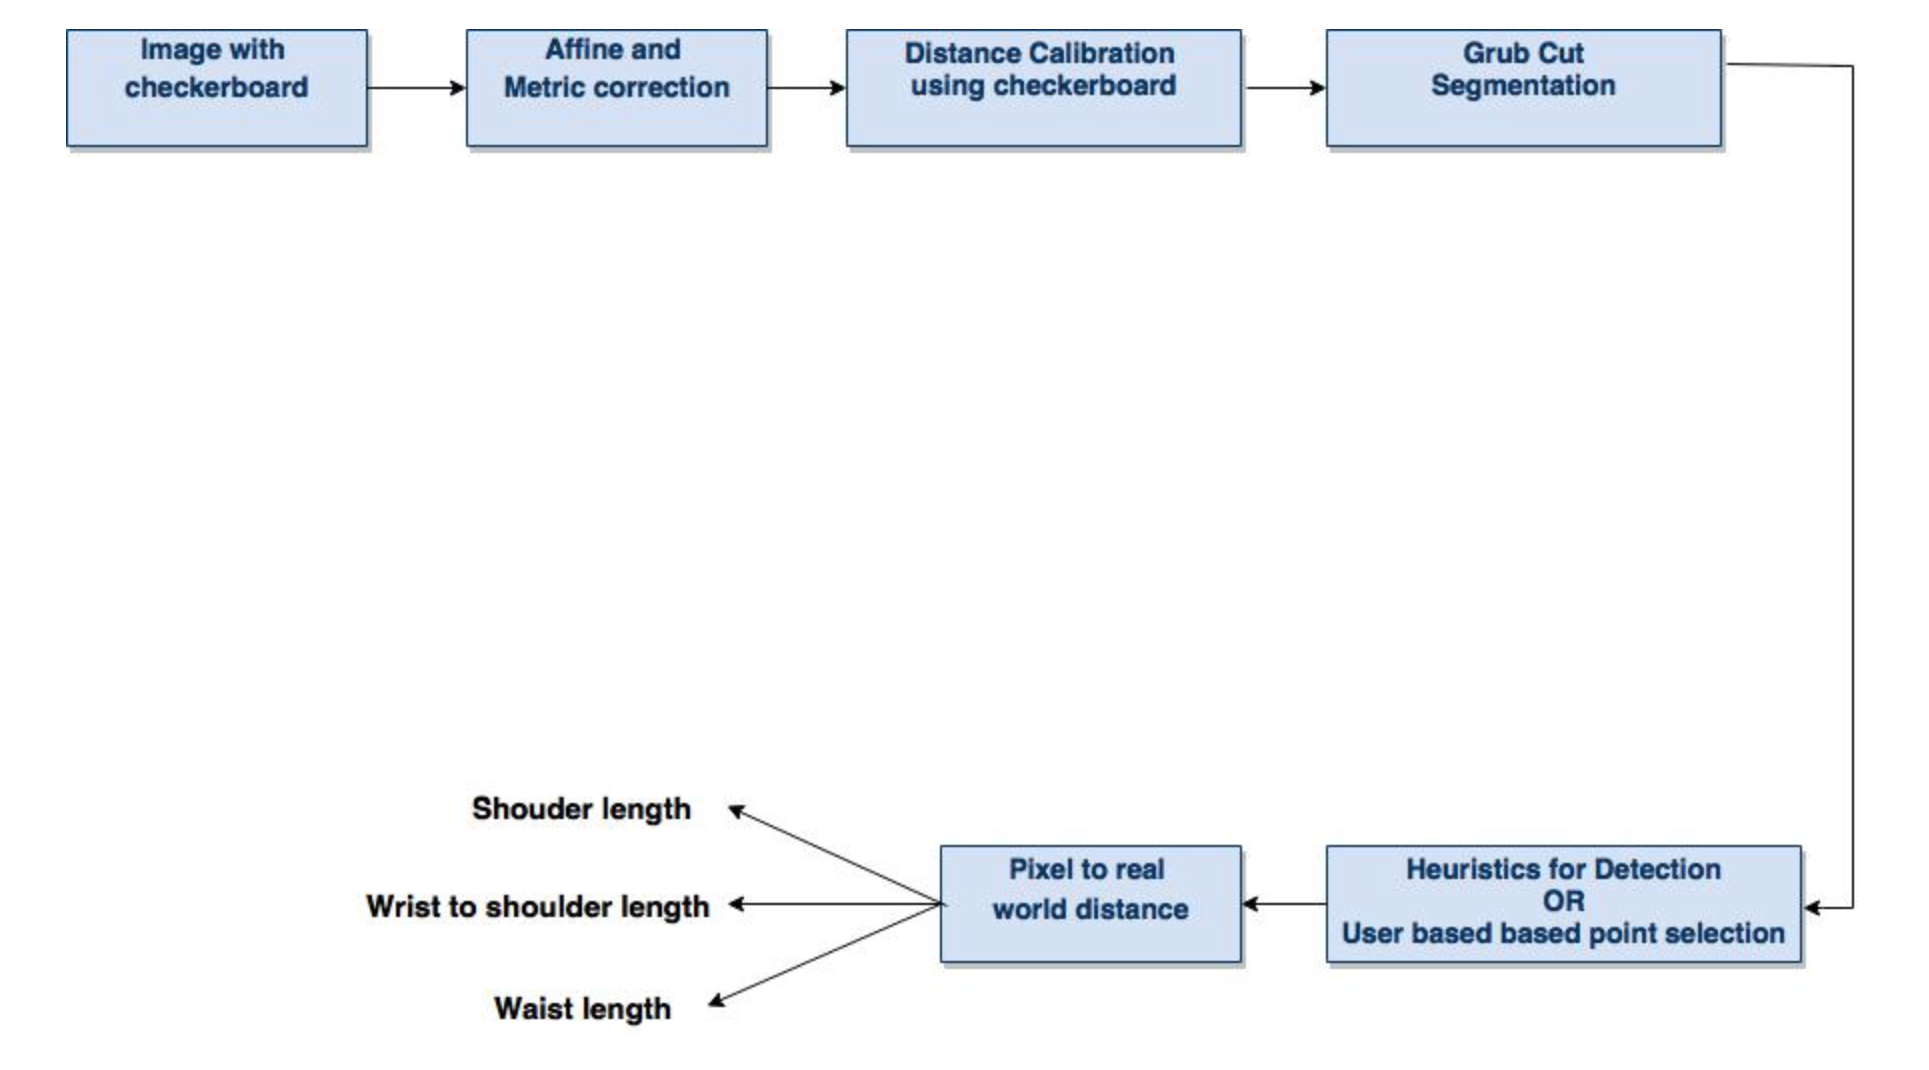
\includegraphics[width=\textwidth]{flow.png}
\end{figure}
\end{frame}

% You can reveal the parts of a slide one at a time
% with the \pause command:
% \begin{frame}{Corrections}
%   \begin{itemize}
%   \item Affine and Metric corrections were performed on input image
  
%   \item We want to completely align(parallel) human body plane and camera image plane(for true measurements).
  
%   \item Subject holds in his hands a checkered board, whose real world distances are known.
  
%   \item Aforementioned corrections were done by automatically detecting a squareboard on the checkered board. 
  
%   \item Image square is then mapped to a correct square ensuring parallelism and perpendicularity in image plane.
 
%   \end{itemize}
% \end{frame}

\begin{frame}{Corrections}
\begin{figure}[h]
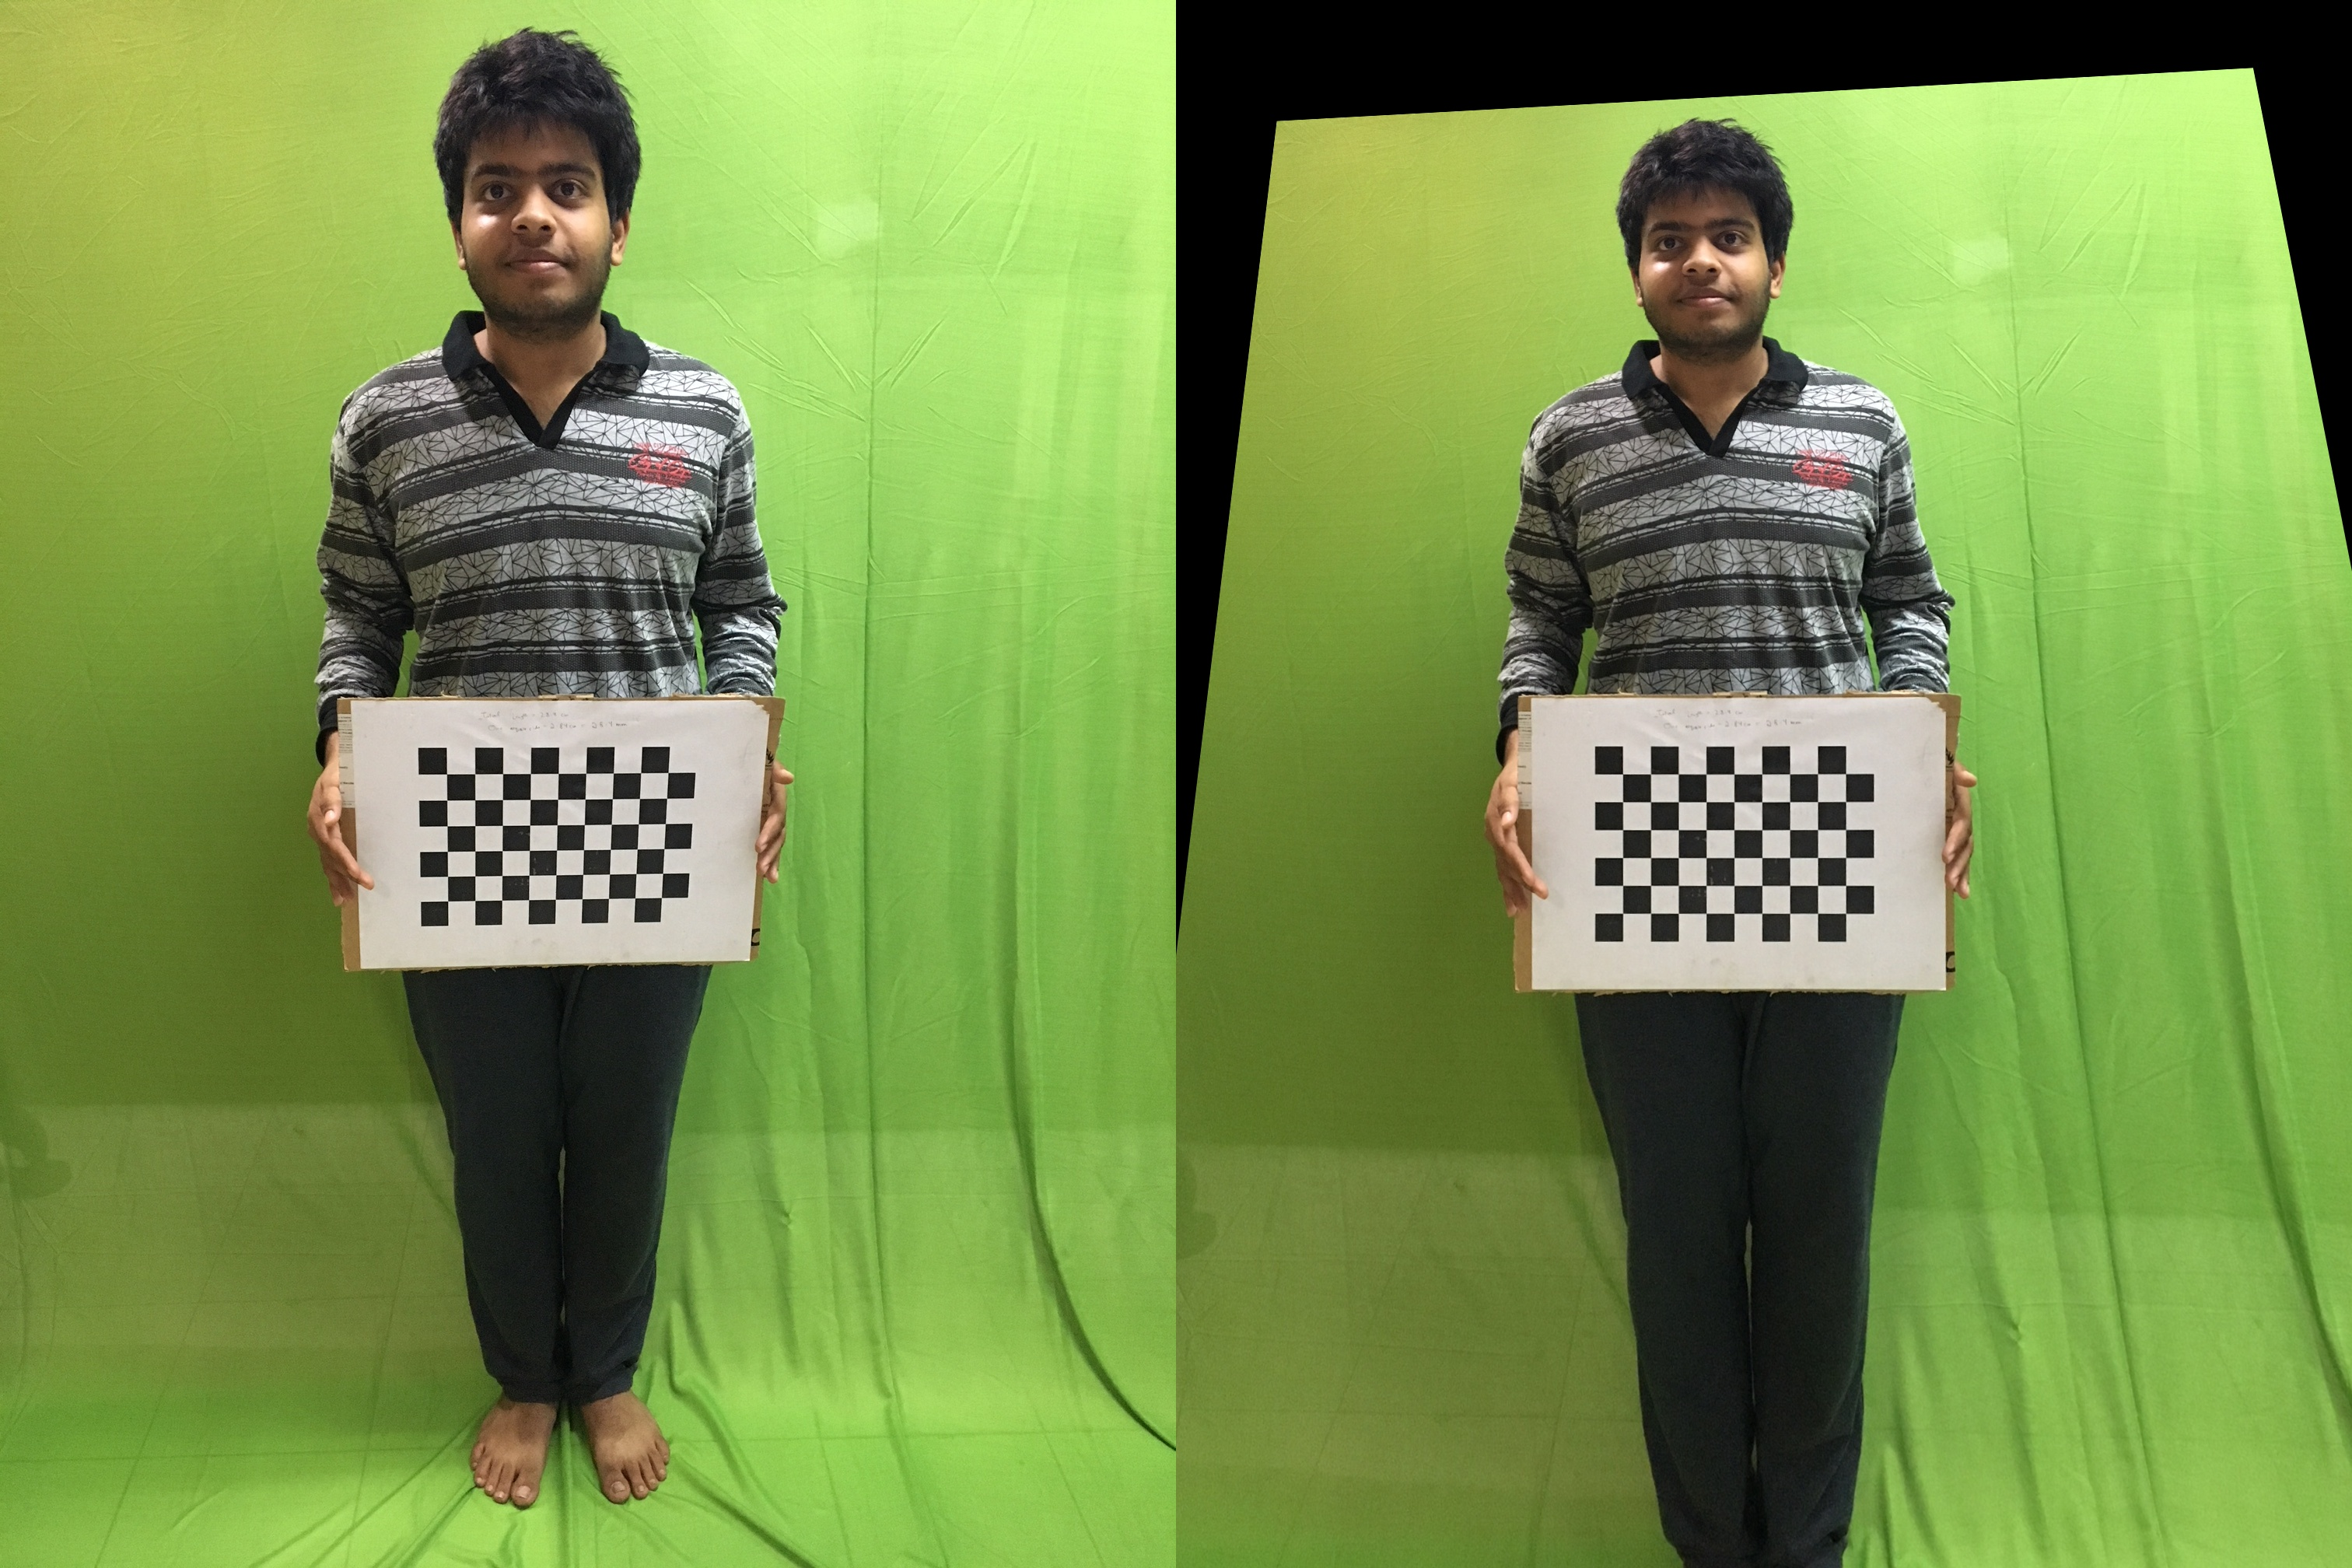
\includegraphics[width=0.9\textwidth]{affine_correction_2.jpg}
\end{figure}
\end{frame}

\begin{frame}{Corrections}
\begin{figure}[h]
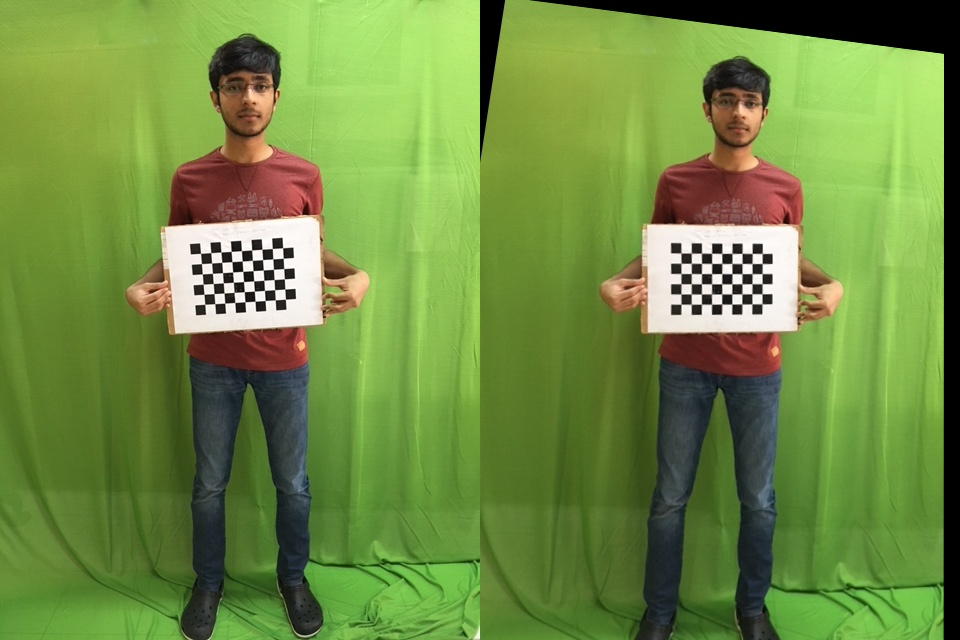
\includegraphics[width=0.9\textwidth]{affine_correction_3.jpg}
\end{figure}
\end{frame}



% \begin{frame}[t]{Unsuccessful Segmentation Attemps}

% \textbf{HaarCascade}
% \begin{itemize}
%     \item It is a machine learning based approach where a cascade function is trained from a lot of positive and negative images. It is then used to detect objects in other images.
% \end{itemize}
% \begin{figure}[h]
%     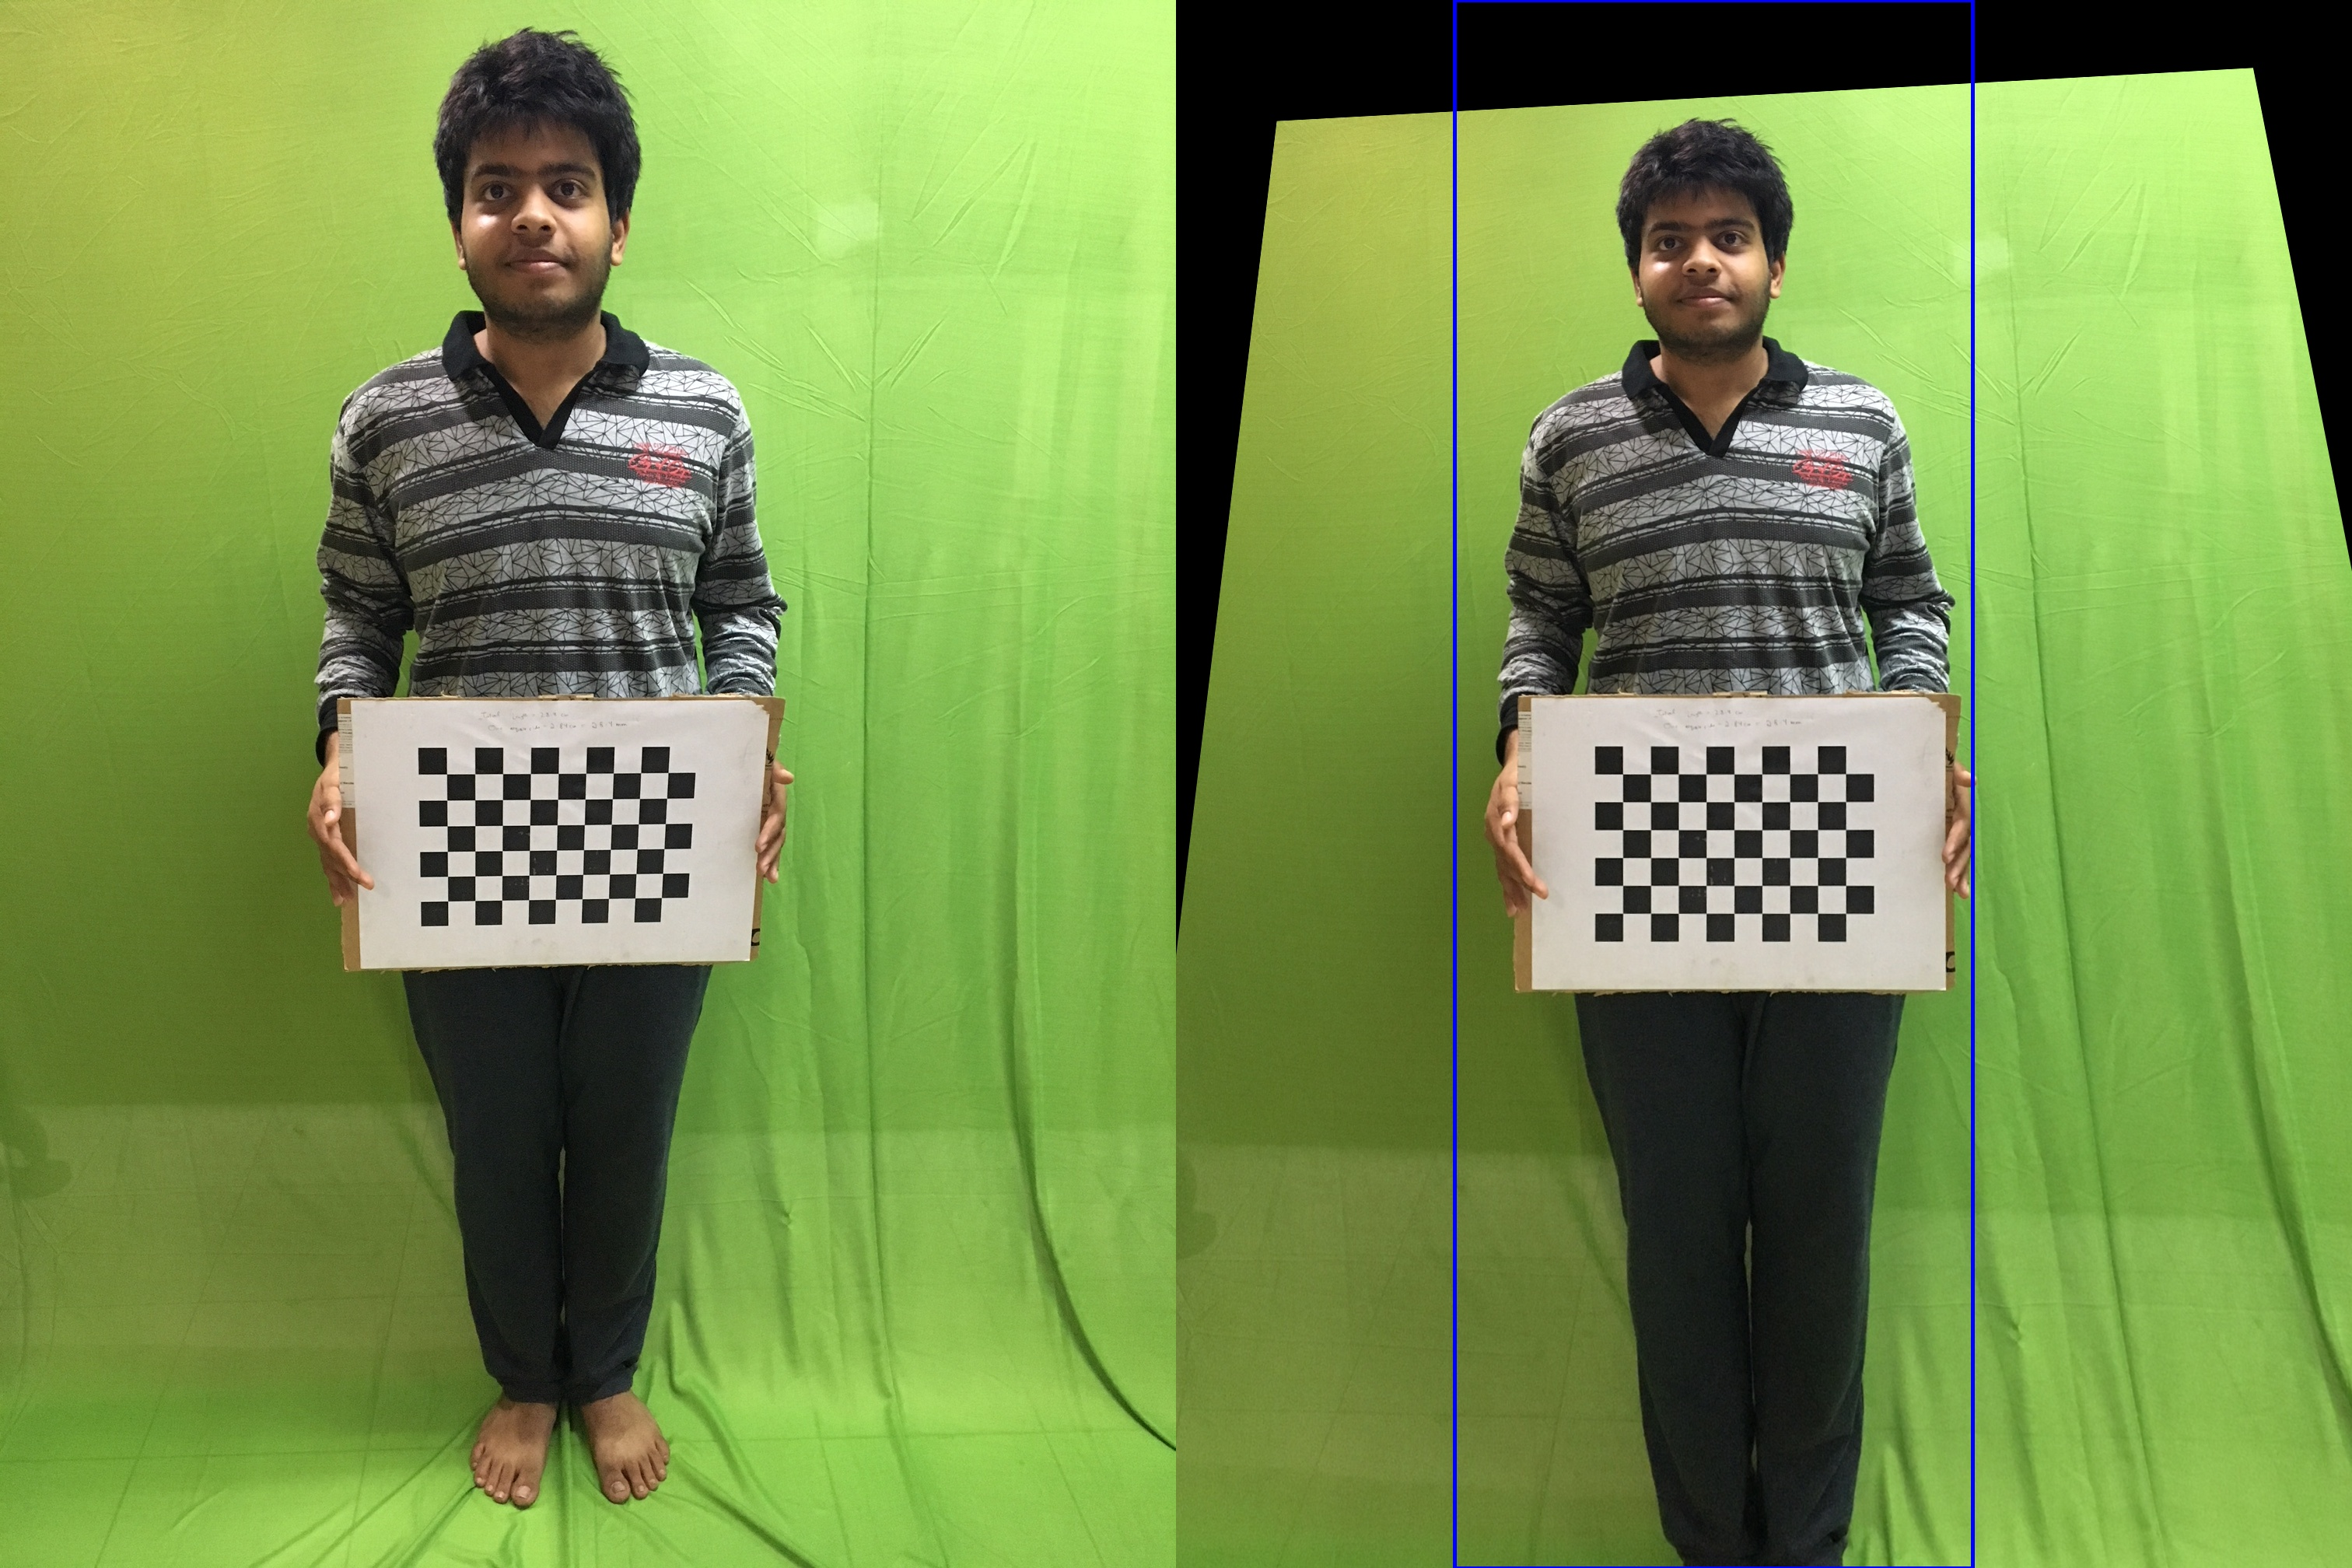
\includegraphics[width=0.7\textwidth]{cascade1.jpg}
% \end{figure}
% \end{frame}    

\begin{frame}[t]{Unsuccessful Segmentation Approach}

\textbf{Grab Cut}
\begin{itemize}
    \item It receives a bounding box and image as input and segments it iteratively. 
    \item It uses color data modelling by iterative energy minimization.
    \item Iterations are extremely slow.
\end{itemize}
\begin{figure}[h]
    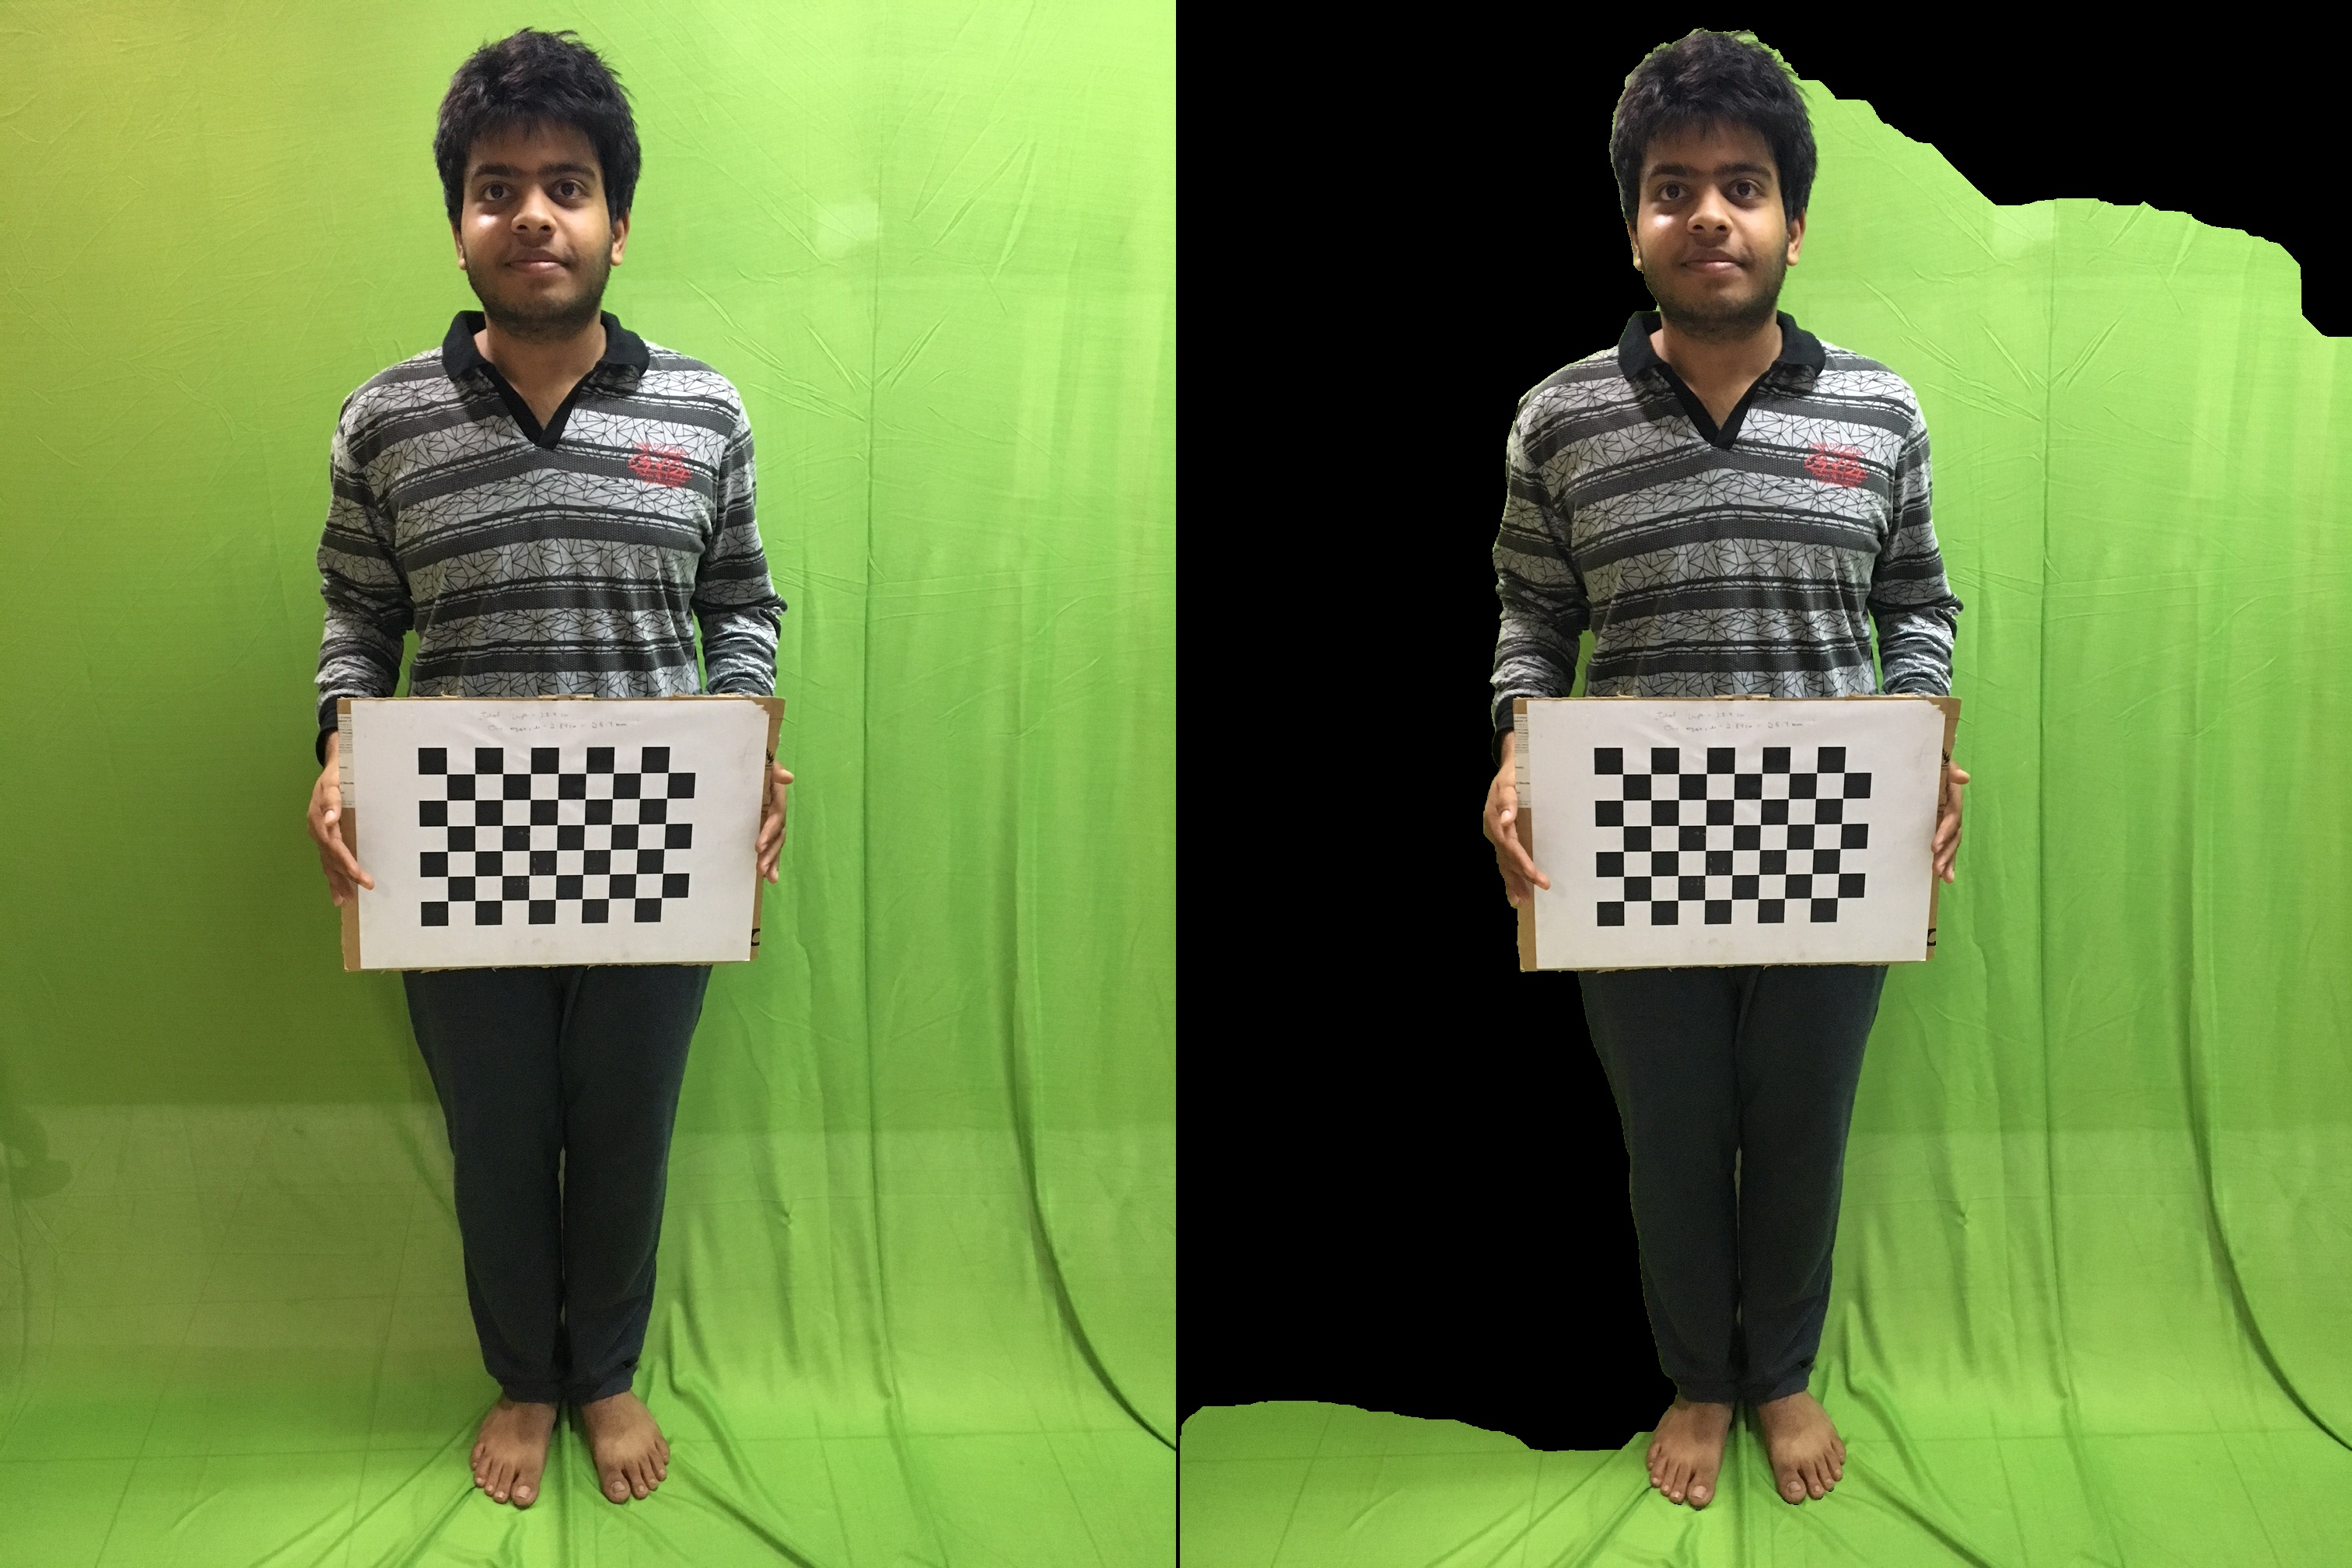
\includegraphics[width=0.6\textwidth]{grub_cut_3.jpg}
\end{figure}
\end{frame}    

\begin{frame}[t]{Green Screen Segmentation}
\begin{itemize}
\item Chroma King technique was used. It segments image based on provided color. 
\item Credits to our Virtual Studio project group for their source code for the same.
\end{itemize}
\begin{figure}[h]
    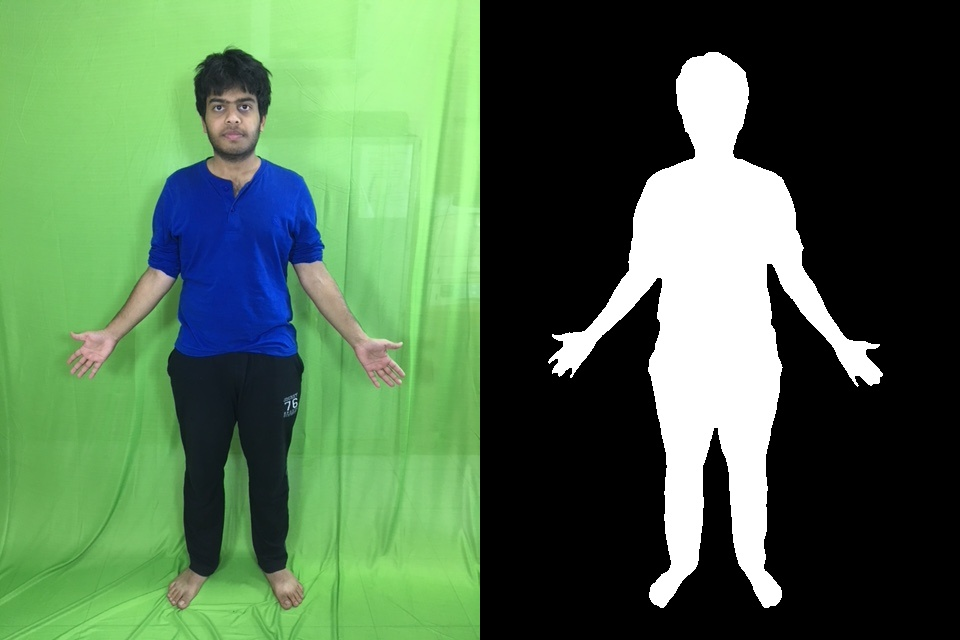
\includegraphics[width=0.65\textwidth]{second.jpg}
\end{figure}
\end{frame}


\begin{frame}[t]{Heuristics to automate point selection}
\textbf{Starting from the segmented image of the human silhouette} \\
\smallskip
\quad \textbf{For shoulder points}
\begin{itemize}
    \item We first find the tip of the head as the highest point in the silhouette
    \item We then move along the horizontal directions from the tip and stop at the point where there is a drastic change in the slope in a window, giving us the shoulder tips
\end{itemize}
\smallskip
\quad We further use a similar heuristic for the wrist points. \\
\smallskip
\quad \textbf{Approximating the waist from two images}
\begin{itemize}
    \item We approximate the waist of the human body as an ellipse
    \item We calculate the semi axis of the ellipse from two images where the person is facing the camera in one image and orthogonal in another
\end{itemize}
\end{frame}


\begin{frame}[t]{Heuristics to automate point selection}
\begin{figure}[h]
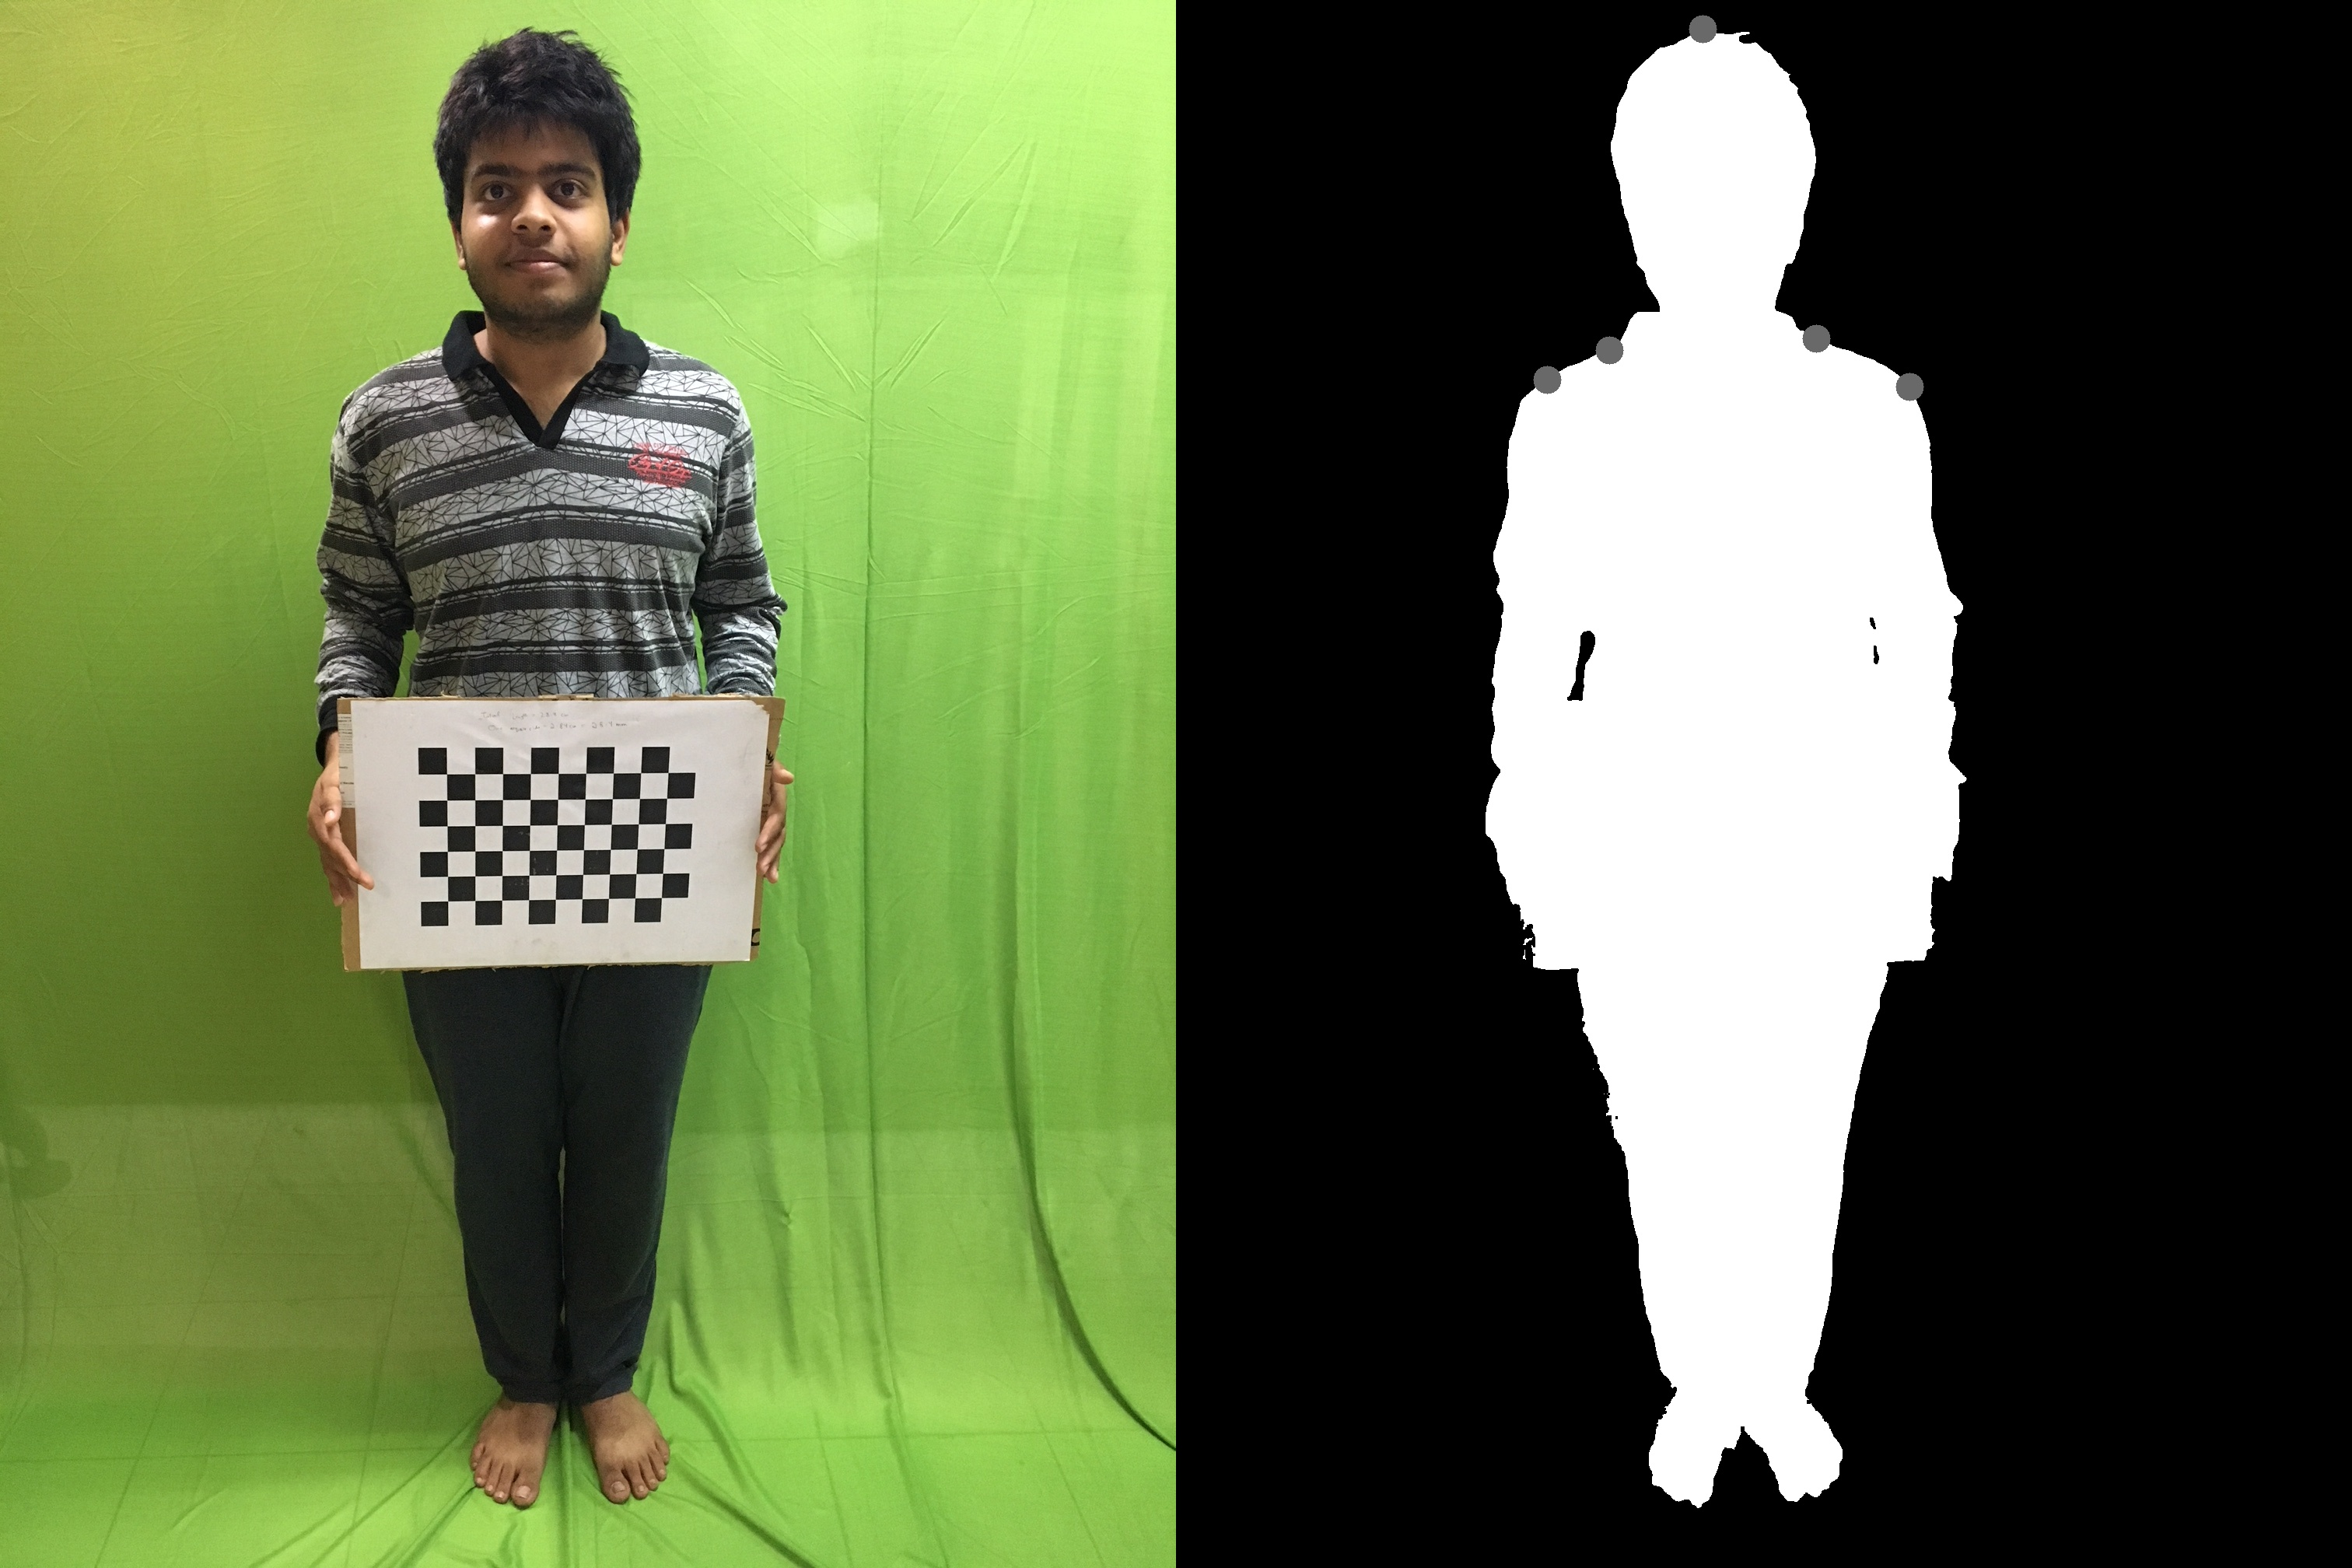
\includegraphics[width=\textwidth]{detected_r.jpg}
\end{figure}
\end{frame}


\begin{frame}{Results}
\begin{figure}[h]
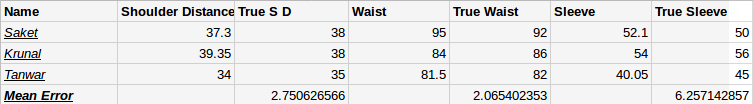
\includegraphics[width=\textwidth]{yeh.png}
\end{figure}
\end{frame}









\begin{frame}{Comparison of shoulder measurement with Kinect results}
Our algorithm showed 40cm shoulder width compared to the 33.6cm given by Kinect when the actual measurement was 38cm
\begin{figure}[h]
    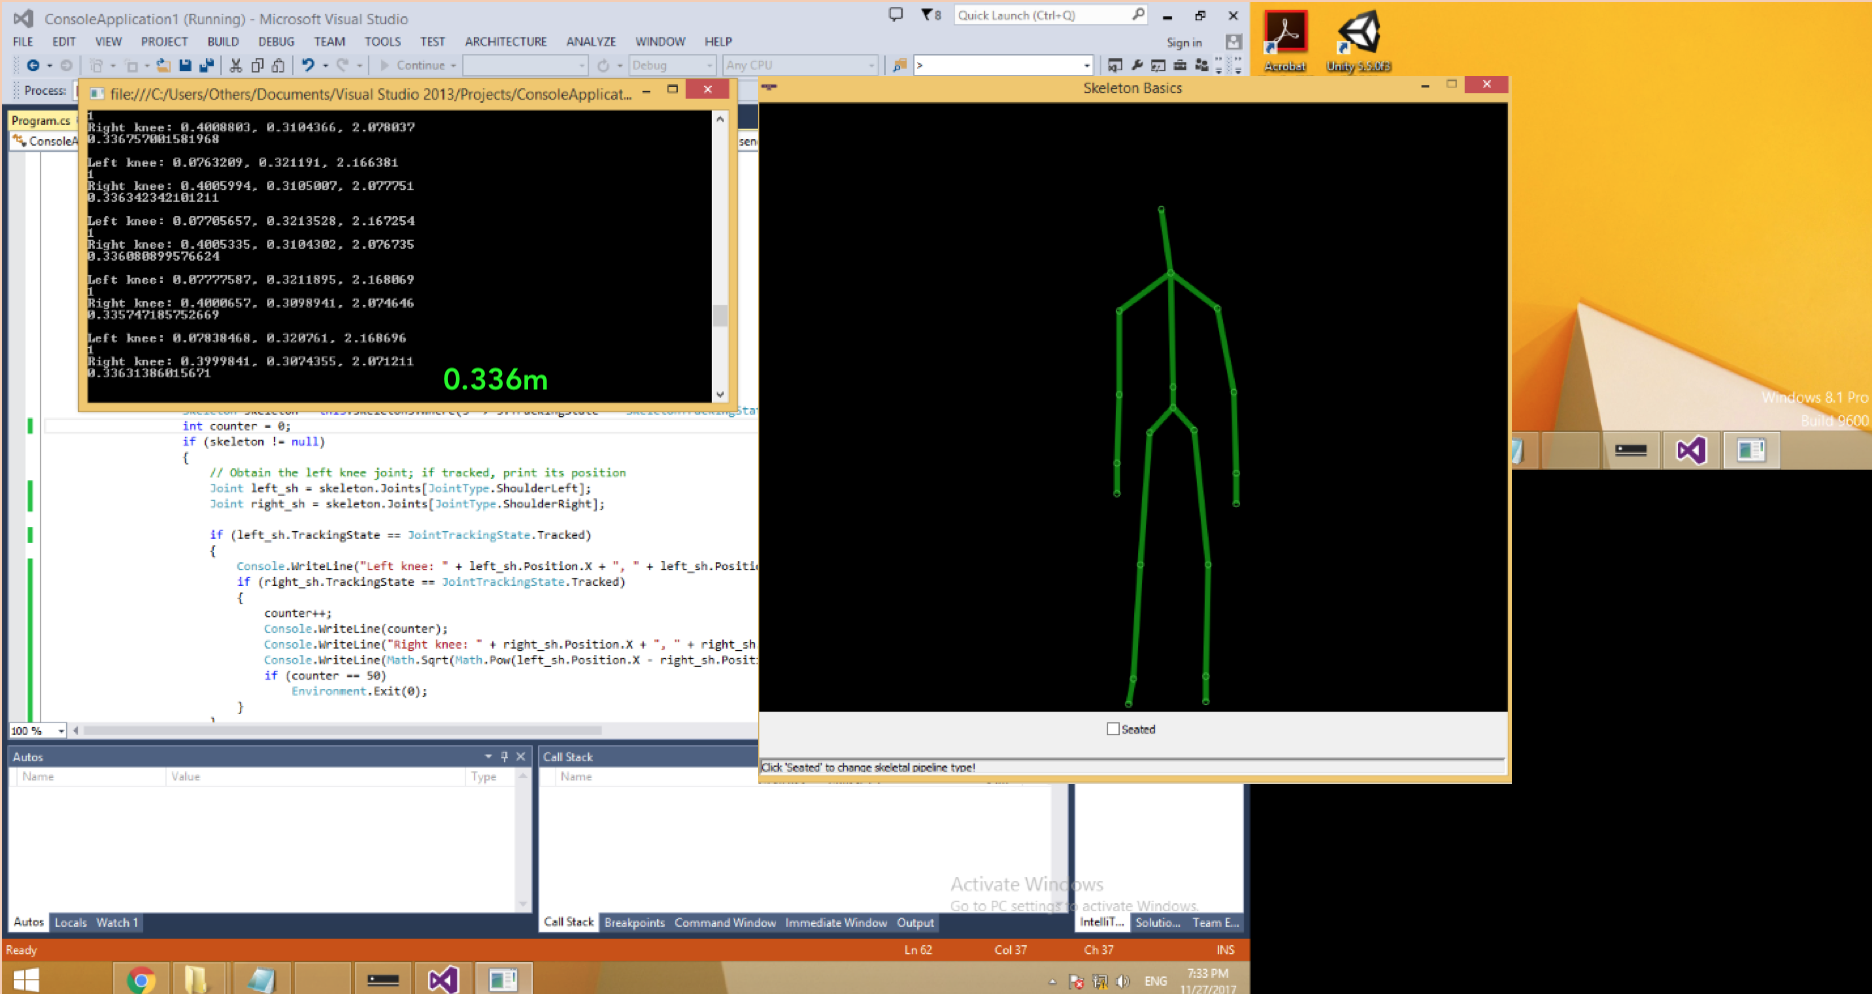
\includegraphics[width=\textwidth]{kinect.png}
\end{figure}
\end{frame}




\begin{frame}{Assumptions}
\begin{itemize}
    \item Since we are trying to approximate the metric rectified images as orthogonal projections we get better results if the human is standing a bit farther from the camera.
    \item We get significantly erroneous results if we try to measure the height using this system since the angles made by the lowermost point with the point of camera centre is large enough to cause significant distortion in the rectified images
    \item The person and the chessboard that the person is holding are approximately parallel and the separation between the two planes is also negligible.
\end{itemize}
\end{frame}



\begin{frame}{Future Scope}
\begin{itemize}
\item Generalizing segmentation - Any background.
\bigskip
\item Robust key-point detection using pose-estimation.
\bigskip
\item Removing dependency from checkerboard and introducing more implicit method for metric calibration.
\end{itemize}
\end{frame}


\end{document}


